\documentclass{article}
\usepackage[margin=2.5cm, top=4cm, headheight=25pt]{geometry}
\usepackage{amsmath, amssymb, enumitem, fancyhdr, graphicx}
\usepackage[indent=20pt]{parskip}
\usepackage[hidelinks]{hyperref}
\usepackage{xcolor}
\usepackage{listings}
\usepackage{subcaption}
\usepackage{url}
\usepackage[most]{tcolorbox}
\usepackage{lastpage}
\usepackage{tikz}
\usepackage{circuitikz}

\usetikzlibrary{arrows, positioning}
\tcbuselibrary{listingsutf8} % Support for lstlistings within tcolorbox

\newtcolorbox[auto counter, number within=section]{question}[1][]{%
    colframe=gray!80,                      % Dark gray frame
    colback=gray!5,                       % Light gray background
    coltitle=black,                        % Black title
    title=\textbf{Question~\thetcbcounter}, % Bold title
    fonttitle=\bfseries\large,             % Subtle title font size
    rounded corners,                   % Slightly more rounded corners
    boxrule=0.25mm,                         % Thinner border for a sleek look
    enhanced,                              % Enhanced box features
    attach boxed title to top left={xshift=2mm, yshift=-2mm},
    boxed title style={colframe=gray!80, colback=gray!5, boxrule=0.25mm},
    % Title styling
    #1
}

\bibliographystyle{IEEEtran}
\graphicspath{{./images/}}

% -- Custom Variables --
\def\me{Group 3}
\def\course{ECE 3760}
\def\labsection{A01}

\def\labno{}
\def\title{Best Physical Design}
% -- Styling for code snippets --
\lstset{
    basicstyle=\ttfamily\scriptsize,           % Basic font style
    keywordstyle=\color{blue},            % Keywords color
    commentstyle=\color{gray},            % Comments color
    stringstyle=\color{teal},             % Strings color
    numbers=left,                         % Line numbers on the left
    numberstyle=\tiny\color{gray},        % Line number style
    stepnumber=1,                         % Line number step
    numbersep=10pt,                       % Space between line numbers and code
    backgroundcolor=\color{lightgray!10}, % Background color
    frame=single,                         % Adds a frame around the code
    breaklines=true,                      % Line breaking for long lines
    captionpos=b,                         % Caption position
    showspaces=false,                     % Don't show spaces
    showstringspaces=false                % Don't show spaces in strings
}
\renewcommand{\lstlistingname}{Code Snippet}

\renewcommand{\arraystretch}{1.2} % For less-ugly tables
\setlength\parindent{0pt}

%----- Samples 
% Questions:
%   \begin{question}[title=Custom Question Title]
%       Question details
%   \end{question}

% Tables:
%   \begin{table}[htbp]
%       \centering
%       \caption{Table Caption}
%       \begin{tabular}{ll}
%           \toprule
%           \textbf{Column 1} & \textbf{Column 2} \\
%           \midrule
%           Row 1 & Row 2 \\
%           Row 3 & Row 4 \\
%           \bottomrule
%       \end{tabular}
%   \end{table} 

% Figures:
%   Single figure:
%       \begin{figure}[htbp]
%           \centering
%           \includegraphics[width=0.5\textwidth]{example-image}
%           \caption{Figure Caption}
%       \end{figure}
%   Multiple figures:
%       \begin{figure}[htbp]
%           \centering
%           \begin{subfigure}[b]{0.5\textwidth}
%               \includegraphics[width=\textwidth]{example-image-a}
%               \caption{First subfigure}
%           \end{subfigure}
%           \begin{subfigure}[b]{0.5\textwidth}
%               \includegraphics[width=\textwidth]{example-image-b}
%               \caption{Second subfigure}
%           \end{subfigure}
%           \caption{Main figure}
%       \end{figure}

\begin{document}

% --------------------------------------------------------------------------------
% TITLE
% --------------------------------------------------------------------------------

\begin{center}
    \huge \title

    \vspace{2mm}
    \hrule

    \vspace{4mm}
    \large \me

    \vspace{2mm}
    \large \course~\labsection

    \vspace{2mm}
    \today
\end{center}

\vspace{4mm}

% --------------------------------------------------------------------------------
% END TITLE
% --------------------------------------------------------------------------------

\newpage


\vspace{1cm}
\newpage

\pagestyle{fancy}
\fancyhead[L]{\large \title}
\fancyhead[R]{\large \me}

\fancyfoot[C]{Page \thepage~of~\pageref{LastPage}}

% --------------------------------------------------------------------------------
% BODY
% --------------------------------------------------------------------------------
\section{Physical Design}
\subsection{Skip and Sweeper Devices}
The skip and sweeper devices share a similar overall design, with the key difference being the top section. The skip device, shown in \autoref{fig:skip_device}, has five larger holes to accommodate buttons for sending commands, while the sweeper device, shown in \autoref{fig:sweeper_device}, has twelve smaller holes arranged in a ring for the LED ring we used as the indicator.

Both devices have a modular design, with identical bottom halves that simplify assembly and reduce manufacturing costs. The top and bottom halves connect via matching screw threads, allowing for easy attachment and replacement if needed. Additionally, each device includes a ring for a lanyard that the skip can use to attach to a neck strap, or belt loop. For the sweeper this is an unecessary feature, but it is included for consistency in design.

\begin{figure}[ht!]
    \centering
    \begin{subfigure}{0.495\textwidth}
        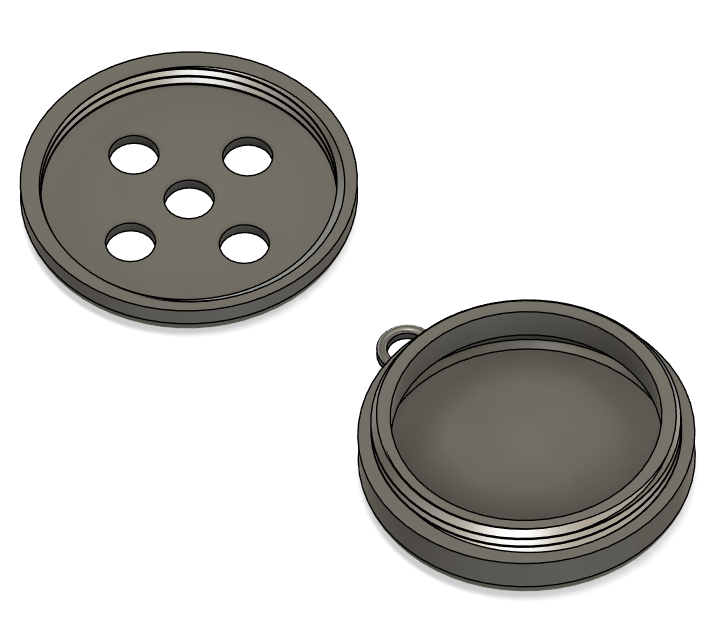
\includegraphics[width=\textwidth]{skip_device.png}
        \caption{Skip Device}
        \label{fig:skip_device}
    \end{subfigure}
    \begin{subfigure}{0.495\textwidth}
        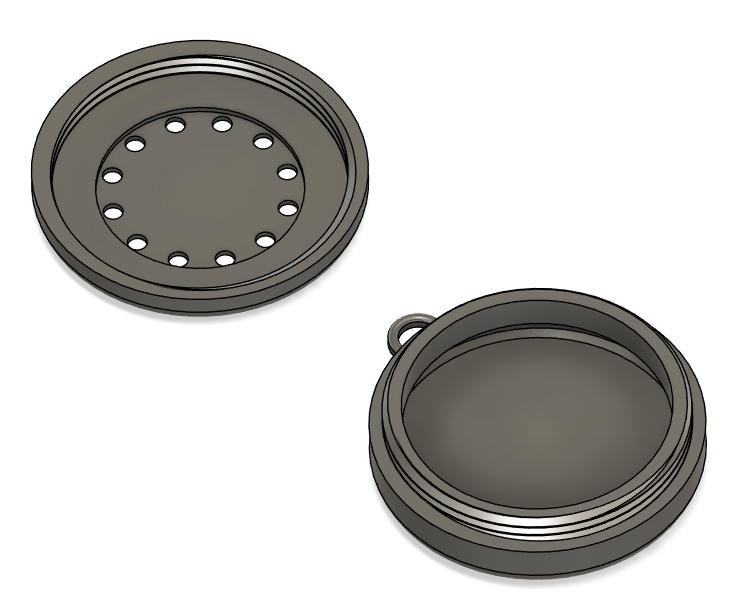
\includegraphics[width=\textwidth]{sweeper_device.png}
        \caption{Sweeper Device}
        \label{fig:sweeper_device}
    \end{subfigure}
    \caption{Skip and Sweeper Devices}
\end{figure}

\subsection{Sweeper Broom Attachment}

The sweeper would slot into the following device seen in \autoref{fig:broom_attachment}. There is a small covering that is attached with some screws, potentially thumb screws so it is easy to remove the sweeper's device. The attachment would clamp onto the broom handle, and the sweeper would be able to posiiton it at any height they prefer. The device is also slightly angled to give the sweeper a better view of the LEDs. This allows us to keep the sweeper device modular, and when charging is required, the attachment can remain on the broom and the device alone can be charge. 

\begin{figure}[ht!]
    \centering
    \begin{subfigure}{0.495\textwidth}
        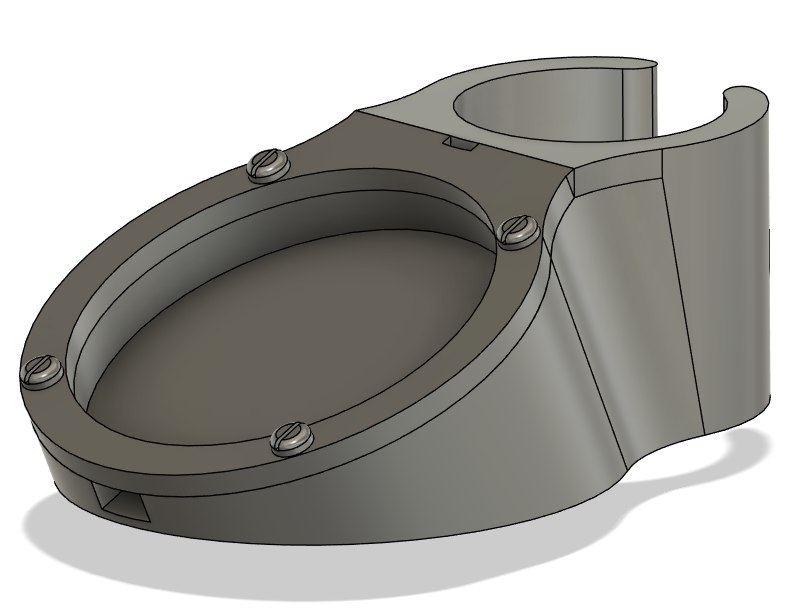
\includegraphics[width=\textwidth]{attachment.png}
        \caption{Broom Attachment}
        \label{fig:broom_attachment}
    \end{subfigure}
    \begin{subfigure}{0.495\textwidth}
        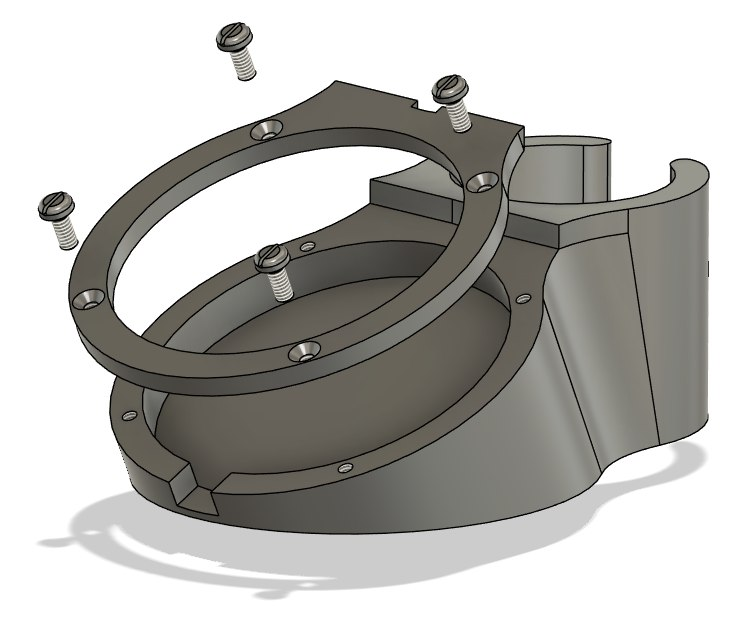
\includegraphics[width=\textwidth]{attachment_exploded.png}
        \caption{Broom Attachment Exploded}
        \label{fig:broom_attachment_side}
    \end{subfigure}
    \caption{Broom Attachment}
\end{figure}



% --------------------------------------------------------------------------------
% END BODY
% --------------------------------------------------------------------------------

\end{document}
